\documentclass[%
fontsize=10%
,a5paper%
,DIV=15%
]{scrartcl}
%scrartcl



\usepackage{gredocument}
\usepackage{psaume}

\title{\centrer{Veillée pascale}}
\author{la nuit de la Résurrection}
\date{avec baptêmes d'adultes}

\makeindex
\definecolor{rubrum}{rgb}{.6,0,0}
\def\rubrum{\color{rubrum}}%%%%%%%mettre"\def\rubrum{\color{rubrum}}" pour avoir le texte adéquat en rouge
\def\nigra{\color{black}}
%    \redlines
%    \definecolor{gregoriocolor}{rgb}{.6,0,0}
%
%\let\red\rubrum

\begin{document}


\maketitle

\newfontfamily\lettrines[Scale=1.3]{LettrinesPro800}
    \def\gretextformat#1{{\fontsize{\taillepolice}{\taillepolice}\selectfont #1}}
    \def\greinitialformat#1{{\lettrines #1}}

\titre{Bénédiction du feu et du cierge}
\vspace{0.5cm}
\rubrica{Le Christ, "lumière du monde" (Jn,8,12) va illuminer tout homme cette nuit en sortant du tombeau, il va dissiper les ténèbres du péché}
\rubrica{Le prête bénit le feu, puis trace sur le cierge la croix, l'alpha et l'oméga, et les chiffres de l'année}
\begin{center}
\versio{Christus Heri et hodie}{Le Christ hier et aujourd'hui}
\versio{Princ\'ipium et Finis}{Commencement et Fin}
\versio{Alpha et Omega}{Alpha et Omega}
\versio{Ips\'ius sunt témpora et s\'æcula}{A lui sont les temps et les siècles}
\versio{Ipsi glória et impérium}{A Lui gloire et domination}
\versio{per univérsa aeternit\'atis s\'æcula. Amen}{pendant tous les siècles de l'éternité. Amen}
\end{center}

\titre{Procession du cierge pascal}
\rubrica{Par trois fois le prêtre annonce la lumière qui jaillit, nous répondons pour manifester notre foi en Dieu, Père, Fils et Saint-Esprit}
\versio{Lumen Christi !}{Lumière du Christ !}
\versio{\textbf{Deo Gratias !}}{\textbf{Nous rendons grâce à Dieu !}}

\rubrica{Alors la Lumière se répand par étape à travers toute l'église en allumant nos cierges au cierge bénit}

\titre{Exsultet}
\rubrica{Alors le prêtre chante l'\emph{Exsultet}, chant de gloire et d'honneur à Jésus, Roi éternel, Lumière du monde, et Vainqueur des ténèbres.}
Qu'elle bondisse de joie, la multitude
des \emph{Anges} dans le ciel!
Qu'ils exultent, ces serviteurs de Dieu !
Et pour la victoire d'un si grand Roi,
que retentisse la trompette sacrée !

Que se réjouisse aussi \emph{la terre},
irradiée de si vives clartés : qu'illuminée par la splendeur du Roi éternel,
elle se sente dégagée des ténèbres
qui couvraient l'univers!

Que se réjouisse aussi notre mère
\emph{l'Eglise}, parée des rayons d'une telle
lumière! Et que cette enceinte résonne
sous les voix puissantes des fidèles!

\cantus{Autre}{PerOmnia-ferial}{}{}

IL est vraiment juste et nécessaire
de faire servir nos voix à célébrer,
de toute l'affection du coeur et de
l'âme, le Dieu invisible, Père toutpuissant,
et son Fils unique notre Seigneur Jésus·Christ, qui a payé d'Adam, et effacé de son sang précieux l'arrêt de l'antique péché.

0 admirable grandeur de votre tendresse envers nous! 0 faveur inestimable de votre
amour : pour délivrer l'esclave, vous livrez le Fils !
0 péché d'Adam qui devait se commettre pour être effacé par la mort du Christ!
\emph{0 heureuse faute qui nous a valu d'avoir un tel, un si grand Rédempteur !}


\titre{Les Lectures}


%\begin{center}
%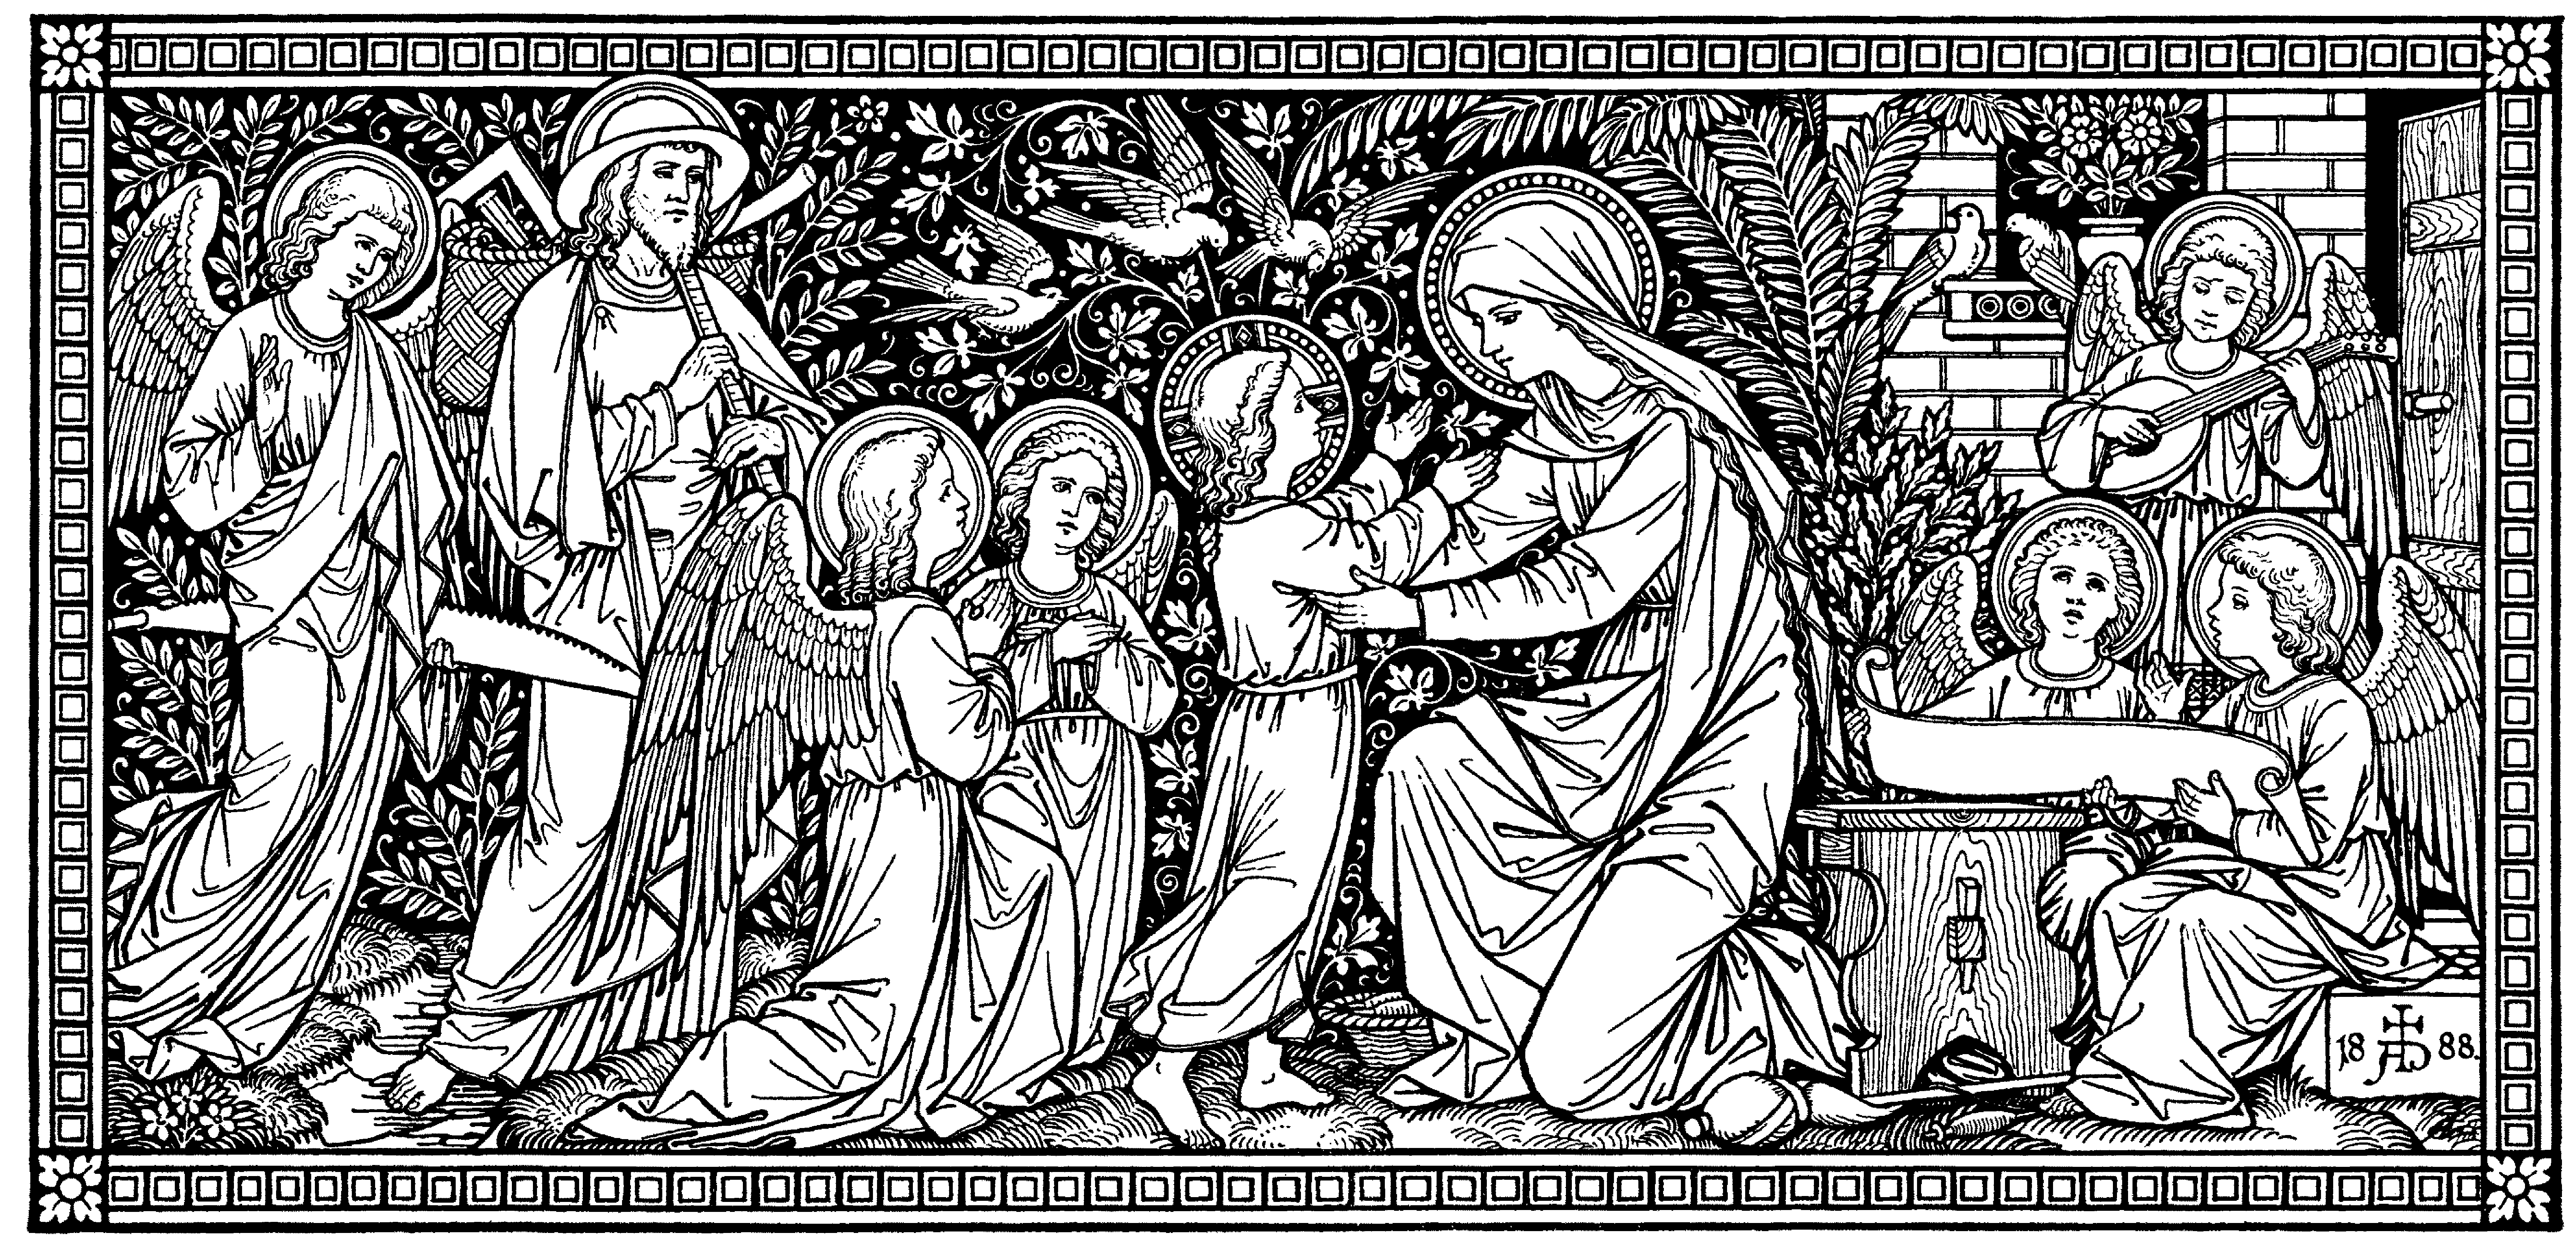
\includegraphics[height=5.5cm]{images/SainteFamille}
%\end{center}





\end{document}